%% figures/fig-regime.tex -- Figure for Sec. 6.3.
%% Pulled into notes.tex with %% figures/fig-regime.tex -- Figure for Sec. 6.3.
%% Pulled into notes.tex with %% figures/fig-regime.tex -- Figure for Sec. 6.3.
%% Pulled into notes.tex with %% figures/fig-regime.tex -- Figure for Sec. 6.3.
%% Pulled into notes.tex with \input{figures/fig-regime}.
%% Needs pgfplots, loaded in the main preamble.
%%
%% The (B, gamma) plane in log-log. Every boundary below is a computed number,
%% not a drawn one; the arithmetic is in the appendix of REVIEW_2026.md and
%% reproduced here:
%%
%%   B_S   = m^2 c^3 / (e hbar) = 4.414e13 G      log10 = 13.645
%%   B_cl  = m^2 c^4 / e^3      = 6.049e15 G      log10 = 15.782  ( = B_S/alpha )
%%   gamma B at tau_0 gamma omega_B = 1 : 3 m^2 c^4 / (2 e^3) = 9.073e15 G
%%                                                   log10 = 15.958
%%
%% Lines of constant gamma*B are straight with slope -1 here:
%%   chi = 0.1        log10 gamma = 12.645 - log10 B
%%   chi = 1          log10 gamma = 13.645 - log10 B
%%   tau_0 g w_B = 1  log10 gamma = 15.958 - log10 B
%% The last two are separated by a factor 3/(2 alpha) = 205.6, i.e. 2.31 decades.
%%
%% Laser point: a0 = 10 at 800 nm gives a lab field 1.34e9 G; head-on the
%% electron sees 2E = 2.68e9 G (log10 = 9.428), so with gamma = 1500
%% (log10 = 3.176) this is chi = 2 gamma E / B_S = 0.091.

\begin{figure}[htb]
\centering
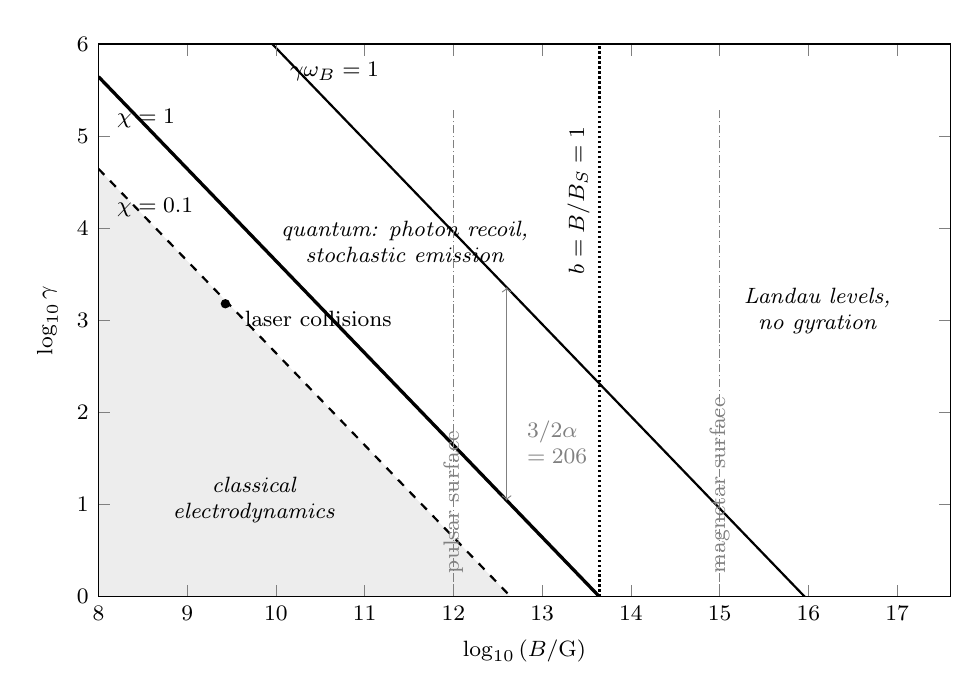
\begin{tikzpicture}
\begin{axis}[
  width=12.4cm, height=8.6cm,
  xlabel={$\log_{10}\,(B/\mathrm{G})$},
  ylabel={$\log_{10}\gamma$},
  xmin=8, xmax=17.6, ymin=0, ymax=6,
  xtick={8,9,10,11,12,13,14,15,16,17},
  ytick={0,1,2,3,4,5,6},
  axis on top, clip=true, samples=2, font=\footnotesize,
  legend style={draw=none,fill=none},
]

  %% ---- the classical wedge: below chi = 0.1 and left of B = B_S ----
  \fill[gray!14]
    (axis cs:8,0) -- (axis cs:8,4.645) -- (axis cs:12.645,0) -- cycle;

  %% ---- Landau quantization: B = B_S, vertical ----
  \addplot[thick,densely dotted,domain=0:6] coordinates {(13.645,0) (13.645,6)};
  \node[rotate=90,anchor=south,font=\footnotesize]
       at (axis cs:13.645,4.30) {$b=B/B_S=1$};

  %% ---- chi = 1 and chi = 0.1 ----
  \addplot[very thick,domain=8:17] {13.645 - x};
  \node[anchor=west,font=\footnotesize] at (axis cs:8.10,5.19) {$\chi=1$};

  \addplot[thick,dashed,domain=8:17] {12.645 - x};
  \node[anchor=west,font=\footnotesize] at (axis cs:8.10,4.22) {$\chi=0.1$};

  %% ---- classical radiation reaction becomes non-perturbative ----
  \addplot[thick,domain=8:17] {15.958 - x};
  \node[anchor=west,font=\footnotesize] at (axis cs:10.05,5.70)
       {$\taunought\gamma\omega_B=1$};

  %% ---- the gap between those two parallel lines, drawn where both are in view
  %%      at x = 12.6 they sit at y = 1.045 and y = 3.358 ----
  \draw[<->,gray] (axis cs:12.6,1.045) -- (axis cs:12.6,3.358);
  \node[anchor=west,font=\footnotesize,gray,align=left]
       at (axis cs:12.72,1.68) {$3/2\alpha$\\$=206$};

  %% ---- regime labels ----
  \node[font=\footnotesize\itshape,align=center] at (axis cs:9.75,1.05)
       {classical\\electrodynamics};
  \node[font=\footnotesize\itshape,align=center] at (axis cs:11.45,3.85)
       {quantum: photon recoil,\\stochastic emission};
  \node[font=\footnotesize\itshape,align=center] at (axis cs:16.1,3.1)
       {Landau levels,\\no gyration};

  %% ---- where things sit ----
  \fill (axis cs:9.43,3.18) circle (1.7pt);
  \node[anchor=west,font=\footnotesize] at (axis cs:9.54,3.02)
       {laser collisions};
  \draw[gray,densely dashdotted] (axis cs:12,0) -- (axis cs:12,5.3);
  \node[rotate=90,anchor=west,font=\footnotesize,gray]
       at (axis cs:12,0.15) {pulsar surface};
  \draw[gray,densely dashdotted] (axis cs:15,0) -- (axis cs:15,5.3);
  \node[rotate=90,anchor=west,font=\footnotesize,gray]
       at (axis cs:15,0.15) {magnetar surface};

\end{axis}
\end{tikzpicture}
\caption{Where classical electrodynamics applies. Shaded is the region in which
it does: $\chi\lesssim0.1$ and $B\lesssim B_S$. Crossing \emph{upward or to the
right} across any boundary leaves it, and the three boundaries fail in
different ways. Above $\chi=1$ a single photon carries a sizeable part of the
particle's energy, so the emission is quantum and stochastic. To the right of
$B=B_S$ the transverse motion is Landau quantized and there is no gyration for
an equation of motion to describe. The line $\taunought\gamma\omega_B=1$ is
where classical radiation reaction would itself become non-perturbative, which
is the regime Secs.~\ref{sec:lorentz} to \ref{sec:eliezer} are about --- and it
lies a factor $3/2\alpha=206$ above the line where the classical description of
the emission has already failed, so it is never reached. Laser--electron
collisions sit at $\chi\approx0.09$ for $a_0=10$ at $800$\,nm against a
$\gamma=1500$ beam, the relevant field being the $2\gamma E$ seen head-on, just inside the classical region and close enough to the
boundary to test it. Pulsar and magnetar surface fields are marked; at a
magnetar surface even a mildly relativistic electron is already past both
quantum boundaries.
\label{fig:regime}}
\end{figure}
.
%% Needs pgfplots, loaded in the main preamble.
%%
%% The (B, gamma) plane in log-log. Every boundary below is a computed number,
%% not a drawn one; the arithmetic is in the appendix of REVIEW_2026.md and
%% reproduced here:
%%
%%   B_S   = m^2 c^3 / (e hbar) = 4.414e13 G      log10 = 13.645
%%   B_cl  = m^2 c^4 / e^3      = 6.049e15 G      log10 = 15.782  ( = B_S/alpha )
%%   gamma B at tau_0 gamma omega_B = 1 : 3 m^2 c^4 / (2 e^3) = 9.073e15 G
%%                                                   log10 = 15.958
%%
%% Lines of constant gamma*B are straight with slope -1 here:
%%   chi = 0.1        log10 gamma = 12.645 - log10 B
%%   chi = 1          log10 gamma = 13.645 - log10 B
%%   tau_0 g w_B = 1  log10 gamma = 15.958 - log10 B
%% The last two are separated by a factor 3/(2 alpha) = 205.6, i.e. 2.31 decades.
%%
%% Laser point: a0 = 10 at 800 nm gives a lab field 1.34e9 G; head-on the
%% electron sees 2E = 2.68e9 G (log10 = 9.428), so with gamma = 1500
%% (log10 = 3.176) this is chi = 2 gamma E / B_S = 0.091.

\begin{figure}[htb]
\centering
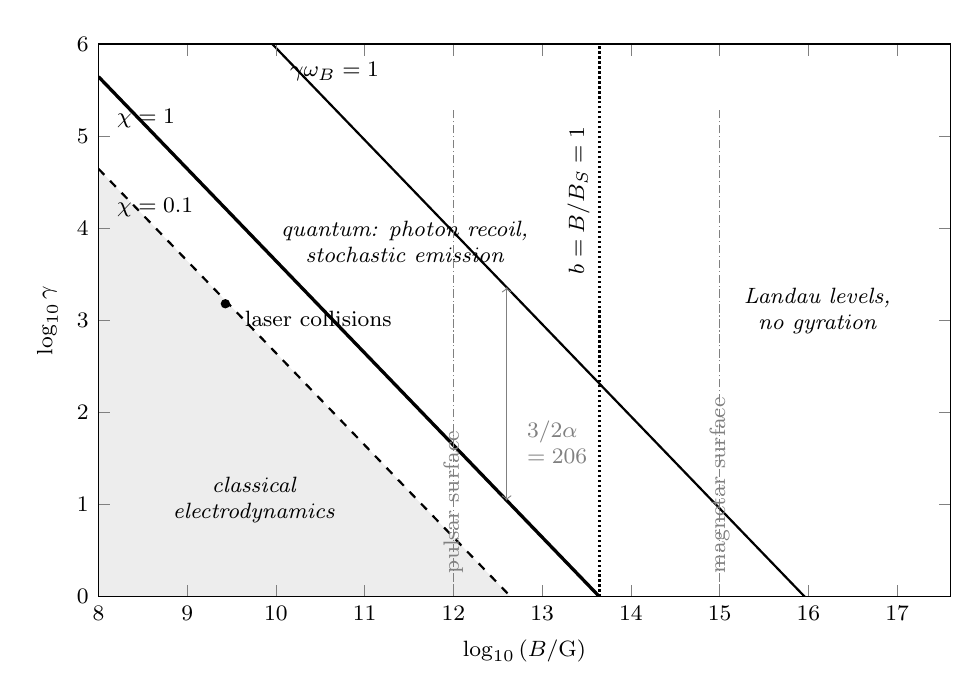
\begin{tikzpicture}
\begin{axis}[
  width=12.4cm, height=8.6cm,
  xlabel={$\log_{10}\,(B/\mathrm{G})$},
  ylabel={$\log_{10}\gamma$},
  xmin=8, xmax=17.6, ymin=0, ymax=6,
  xtick={8,9,10,11,12,13,14,15,16,17},
  ytick={0,1,2,3,4,5,6},
  axis on top, clip=true, samples=2, font=\footnotesize,
  legend style={draw=none,fill=none},
]

  %% ---- the classical wedge: below chi = 0.1 and left of B = B_S ----
  \fill[gray!14]
    (axis cs:8,0) -- (axis cs:8,4.645) -- (axis cs:12.645,0) -- cycle;

  %% ---- Landau quantization: B = B_S, vertical ----
  \addplot[thick,densely dotted,domain=0:6] coordinates {(13.645,0) (13.645,6)};
  \node[rotate=90,anchor=south,font=\footnotesize]
       at (axis cs:13.645,4.30) {$b=B/B_S=1$};

  %% ---- chi = 1 and chi = 0.1 ----
  \addplot[very thick,domain=8:17] {13.645 - x};
  \node[anchor=west,font=\footnotesize] at (axis cs:8.10,5.19) {$\chi=1$};

  \addplot[thick,dashed,domain=8:17] {12.645 - x};
  \node[anchor=west,font=\footnotesize] at (axis cs:8.10,4.22) {$\chi=0.1$};

  %% ---- classical radiation reaction becomes non-perturbative ----
  \addplot[thick,domain=8:17] {15.958 - x};
  \node[anchor=west,font=\footnotesize] at (axis cs:10.05,5.70)
       {$\taunought\gamma\omega_B=1$};

  %% ---- the gap between those two parallel lines, drawn where both are in view
  %%      at x = 12.6 they sit at y = 1.045 and y = 3.358 ----
  \draw[<->,gray] (axis cs:12.6,1.045) -- (axis cs:12.6,3.358);
  \node[anchor=west,font=\footnotesize,gray,align=left]
       at (axis cs:12.72,1.68) {$3/2\alpha$\\$=206$};

  %% ---- regime labels ----
  \node[font=\footnotesize\itshape,align=center] at (axis cs:9.75,1.05)
       {classical\\electrodynamics};
  \node[font=\footnotesize\itshape,align=center] at (axis cs:11.45,3.85)
       {quantum: photon recoil,\\stochastic emission};
  \node[font=\footnotesize\itshape,align=center] at (axis cs:16.1,3.1)
       {Landau levels,\\no gyration};

  %% ---- where things sit ----
  \fill (axis cs:9.43,3.18) circle (1.7pt);
  \node[anchor=west,font=\footnotesize] at (axis cs:9.54,3.02)
       {laser collisions};
  \draw[gray,densely dashdotted] (axis cs:12,0) -- (axis cs:12,5.3);
  \node[rotate=90,anchor=west,font=\footnotesize,gray]
       at (axis cs:12,0.15) {pulsar surface};
  \draw[gray,densely dashdotted] (axis cs:15,0) -- (axis cs:15,5.3);
  \node[rotate=90,anchor=west,font=\footnotesize,gray]
       at (axis cs:15,0.15) {magnetar surface};

\end{axis}
\end{tikzpicture}
\caption{Where classical electrodynamics applies. Shaded is the region in which
it does: $\chi\lesssim0.1$ and $B\lesssim B_S$. Crossing \emph{upward or to the
right} across any boundary leaves it, and the three boundaries fail in
different ways. Above $\chi=1$ a single photon carries a sizeable part of the
particle's energy, so the emission is quantum and stochastic. To the right of
$B=B_S$ the transverse motion is Landau quantized and there is no gyration for
an equation of motion to describe. The line $\taunought\gamma\omega_B=1$ is
where classical radiation reaction would itself become non-perturbative, which
is the regime Secs.~\ref{sec:lorentz} to \ref{sec:eliezer} are about --- and it
lies a factor $3/2\alpha=206$ above the line where the classical description of
the emission has already failed, so it is never reached. Laser--electron
collisions sit at $\chi\approx0.09$ for $a_0=10$ at $800$\,nm against a
$\gamma=1500$ beam, the relevant field being the $2\gamma E$ seen head-on, just inside the classical region and close enough to the
boundary to test it. Pulsar and magnetar surface fields are marked; at a
magnetar surface even a mildly relativistic electron is already past both
quantum boundaries.
\label{fig:regime}}
\end{figure}
.
%% Needs pgfplots, loaded in the main preamble.
%%
%% The (B, gamma) plane in log-log. Every boundary below is a computed number,
%% not a drawn one; the arithmetic is in the appendix of REVIEW_2026.md and
%% reproduced here:
%%
%%   B_S   = m^2 c^3 / (e hbar) = 4.414e13 G      log10 = 13.645
%%   B_cl  = m^2 c^4 / e^3      = 6.049e15 G      log10 = 15.782  ( = B_S/alpha )
%%   gamma B at tau_0 gamma omega_B = 1 : 3 m^2 c^4 / (2 e^3) = 9.073e15 G
%%                                                   log10 = 15.958
%%
%% Lines of constant gamma*B are straight with slope -1 here:
%%   chi = 0.1        log10 gamma = 12.645 - log10 B
%%   chi = 1          log10 gamma = 13.645 - log10 B
%%   tau_0 g w_B = 1  log10 gamma = 15.958 - log10 B
%% The last two are separated by a factor 3/(2 alpha) = 205.6, i.e. 2.31 decades.
%%
%% Laser point: a0 = 10 at 800 nm gives a lab field 1.34e9 G; head-on the
%% electron sees 2E = 2.68e9 G (log10 = 9.428), so with gamma = 1500
%% (log10 = 3.176) this is chi = 2 gamma E / B_S = 0.091.

\begin{figure}[htb]
\centering
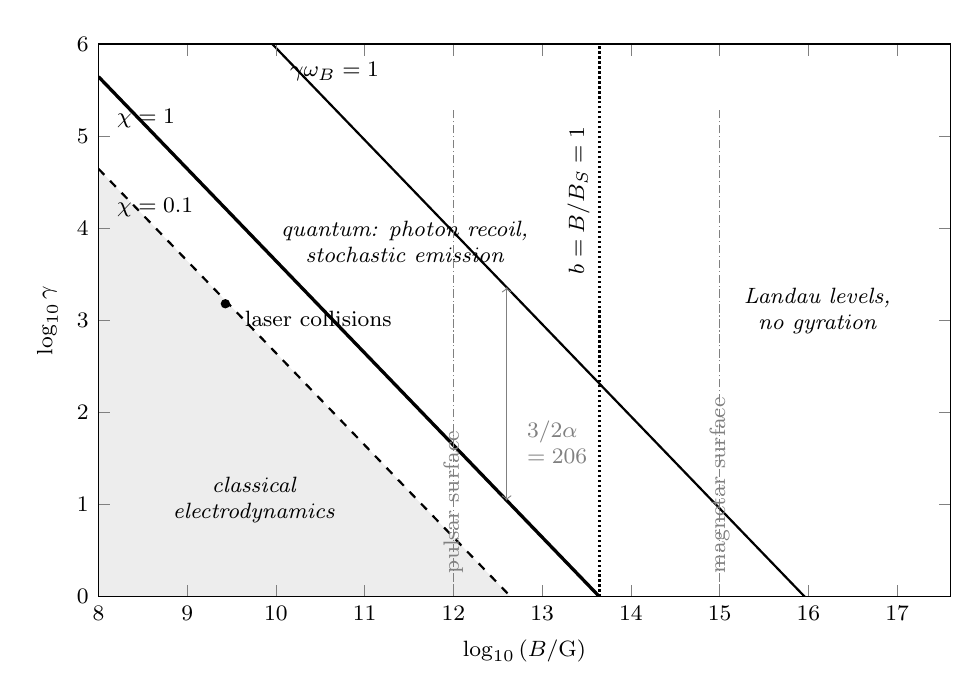
\begin{tikzpicture}
\begin{axis}[
  width=12.4cm, height=8.6cm,
  xlabel={$\log_{10}\,(B/\mathrm{G})$},
  ylabel={$\log_{10}\gamma$},
  xmin=8, xmax=17.6, ymin=0, ymax=6,
  xtick={8,9,10,11,12,13,14,15,16,17},
  ytick={0,1,2,3,4,5,6},
  axis on top, clip=true, samples=2, font=\footnotesize,
  legend style={draw=none,fill=none},
]

  %% ---- the classical wedge: below chi = 0.1 and left of B = B_S ----
  \fill[gray!14]
    (axis cs:8,0) -- (axis cs:8,4.645) -- (axis cs:12.645,0) -- cycle;

  %% ---- Landau quantization: B = B_S, vertical ----
  \addplot[thick,densely dotted,domain=0:6] coordinates {(13.645,0) (13.645,6)};
  \node[rotate=90,anchor=south,font=\footnotesize]
       at (axis cs:13.645,4.30) {$b=B/B_S=1$};

  %% ---- chi = 1 and chi = 0.1 ----
  \addplot[very thick,domain=8:17] {13.645 - x};
  \node[anchor=west,font=\footnotesize] at (axis cs:8.10,5.19) {$\chi=1$};

  \addplot[thick,dashed,domain=8:17] {12.645 - x};
  \node[anchor=west,font=\footnotesize] at (axis cs:8.10,4.22) {$\chi=0.1$};

  %% ---- classical radiation reaction becomes non-perturbative ----
  \addplot[thick,domain=8:17] {15.958 - x};
  \node[anchor=west,font=\footnotesize] at (axis cs:10.05,5.70)
       {$\taunought\gamma\omega_B=1$};

  %% ---- the gap between those two parallel lines, drawn where both are in view
  %%      at x = 12.6 they sit at y = 1.045 and y = 3.358 ----
  \draw[<->,gray] (axis cs:12.6,1.045) -- (axis cs:12.6,3.358);
  \node[anchor=west,font=\footnotesize,gray,align=left]
       at (axis cs:12.72,1.68) {$3/2\alpha$\\$=206$};

  %% ---- regime labels ----
  \node[font=\footnotesize\itshape,align=center] at (axis cs:9.75,1.05)
       {classical\\electrodynamics};
  \node[font=\footnotesize\itshape,align=center] at (axis cs:11.45,3.85)
       {quantum: photon recoil,\\stochastic emission};
  \node[font=\footnotesize\itshape,align=center] at (axis cs:16.1,3.1)
       {Landau levels,\\no gyration};

  %% ---- where things sit ----
  \fill (axis cs:9.43,3.18) circle (1.7pt);
  \node[anchor=west,font=\footnotesize] at (axis cs:9.54,3.02)
       {laser collisions};
  \draw[gray,densely dashdotted] (axis cs:12,0) -- (axis cs:12,5.3);
  \node[rotate=90,anchor=west,font=\footnotesize,gray]
       at (axis cs:12,0.15) {pulsar surface};
  \draw[gray,densely dashdotted] (axis cs:15,0) -- (axis cs:15,5.3);
  \node[rotate=90,anchor=west,font=\footnotesize,gray]
       at (axis cs:15,0.15) {magnetar surface};

\end{axis}
\end{tikzpicture}
\caption{Where classical electrodynamics applies. Shaded is the region in which
it does: $\chi\lesssim0.1$ and $B\lesssim B_S$. Crossing \emph{upward or to the
right} across any boundary leaves it, and the three boundaries fail in
different ways. Above $\chi=1$ a single photon carries a sizeable part of the
particle's energy, so the emission is quantum and stochastic. To the right of
$B=B_S$ the transverse motion is Landau quantized and there is no gyration for
an equation of motion to describe. The line $\taunought\gamma\omega_B=1$ is
where classical radiation reaction would itself become non-perturbative, which
is the regime Secs.~\ref{sec:lorentz} to \ref{sec:eliezer} are about --- and it
lies a factor $3/2\alpha=206$ above the line where the classical description of
the emission has already failed, so it is never reached. Laser--electron
collisions sit at $\chi\approx0.09$ for $a_0=10$ at $800$\,nm against a
$\gamma=1500$ beam, the relevant field being the $2\gamma E$ seen head-on, just inside the classical region and close enough to the
boundary to test it. Pulsar and magnetar surface fields are marked; at a
magnetar surface even a mildly relativistic electron is already past both
quantum boundaries.
\label{fig:regime}}
\end{figure}
.
%% Needs pgfplots, loaded in the main preamble.
%%
%% The (B, gamma) plane in log-log. Every boundary below is a computed number,
%% not a drawn one; the arithmetic is in the appendix of REVIEW_2026.md and
%% reproduced here:
%%
%%   B_S   = m^2 c^3 / (e hbar) = 4.414e13 G      log10 = 13.645
%%   B_cl  = m^2 c^4 / e^3      = 6.049e15 G      log10 = 15.782  ( = B_S/alpha )
%%   gamma B at tau_0 gamma omega_B = 1 : 3 m^2 c^4 / (2 e^3) = 9.073e15 G
%%                                                   log10 = 15.958
%%
%% Lines of constant gamma*B are straight with slope -1 here:
%%   chi = 0.1        log10 gamma = 12.645 - log10 B
%%   chi = 1          log10 gamma = 13.645 - log10 B
%%   tau_0 g w_B = 1  log10 gamma = 15.958 - log10 B
%% The last two are separated by a factor 3/(2 alpha) = 205.6, i.e. 2.31 decades.
%%
%% Laser point: a0 = 10 at 800 nm gives a lab field 1.34e9 G; head-on the
%% electron sees 2E = 2.68e9 G (log10 = 9.428), so with gamma = 1500
%% (log10 = 3.176) this is chi = 2 gamma E / B_S = 0.091.

\begin{figure}[htb]
\centering
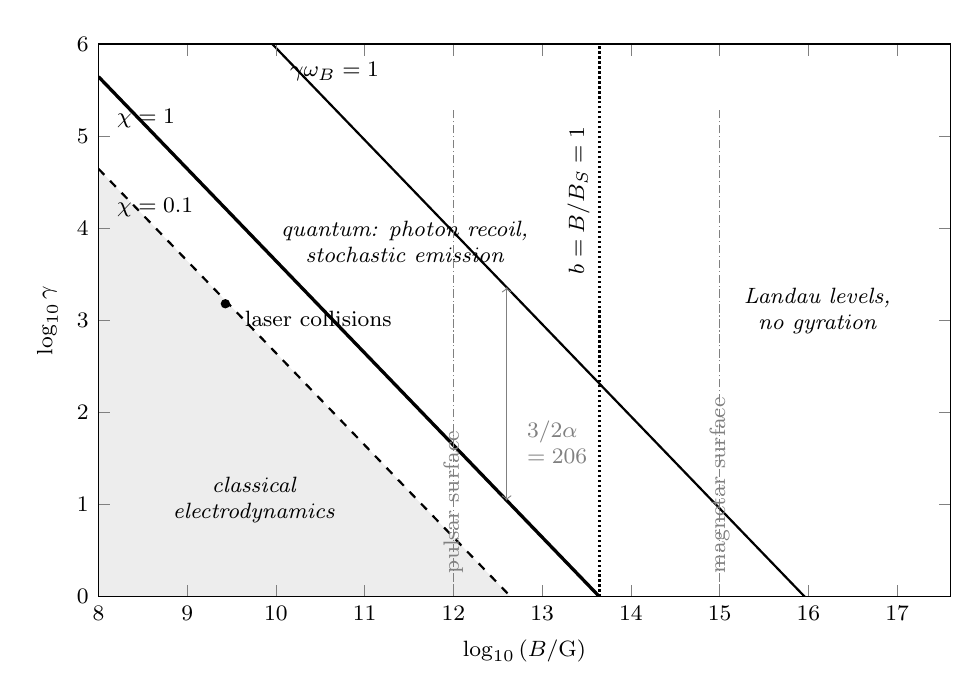
\begin{tikzpicture}
\begin{axis}[
  width=12.4cm, height=8.6cm,
  xlabel={$\log_{10}\,(B/\mathrm{G})$},
  ylabel={$\log_{10}\gamma$},
  xmin=8, xmax=17.6, ymin=0, ymax=6,
  xtick={8,9,10,11,12,13,14,15,16,17},
  ytick={0,1,2,3,4,5,6},
  axis on top, clip=true, samples=2, font=\footnotesize,
  legend style={draw=none,fill=none},
]

  %% ---- the classical wedge: below chi = 0.1 and left of B = B_S ----
  \fill[gray!14]
    (axis cs:8,0) -- (axis cs:8,4.645) -- (axis cs:12.645,0) -- cycle;

  %% ---- Landau quantization: B = B_S, vertical ----
  \addplot[thick,densely dotted,domain=0:6] coordinates {(13.645,0) (13.645,6)};
  \node[rotate=90,anchor=south,font=\footnotesize]
       at (axis cs:13.645,4.30) {$b=B/B_S=1$};

  %% ---- chi = 1 and chi = 0.1 ----
  \addplot[very thick,domain=8:17] {13.645 - x};
  \node[anchor=west,font=\footnotesize] at (axis cs:8.10,5.19) {$\chi=1$};

  \addplot[thick,dashed,domain=8:17] {12.645 - x};
  \node[anchor=west,font=\footnotesize] at (axis cs:8.10,4.22) {$\chi=0.1$};

  %% ---- classical radiation reaction becomes non-perturbative ----
  \addplot[thick,domain=8:17] {15.958 - x};
  \node[anchor=west,font=\footnotesize] at (axis cs:10.05,5.70)
       {$\taunought\gamma\omega_B=1$};

  %% ---- the gap between those two parallel lines, drawn where both are in view
  %%      at x = 12.6 they sit at y = 1.045 and y = 3.358 ----
  \draw[<->,gray] (axis cs:12.6,1.045) -- (axis cs:12.6,3.358);
  \node[anchor=west,font=\footnotesize,gray,align=left]
       at (axis cs:12.72,1.68) {$3/2\alpha$\\$=206$};

  %% ---- regime labels ----
  \node[font=\footnotesize\itshape,align=center] at (axis cs:9.75,1.05)
       {classical\\electrodynamics};
  \node[font=\footnotesize\itshape,align=center] at (axis cs:11.45,3.85)
       {quantum: photon recoil,\\stochastic emission};
  \node[font=\footnotesize\itshape,align=center] at (axis cs:16.1,3.1)
       {Landau levels,\\no gyration};

  %% ---- where things sit ----
  \fill (axis cs:9.43,3.18) circle (1.7pt);
  \node[anchor=west,font=\footnotesize] at (axis cs:9.54,3.02)
       {laser collisions};
  \draw[gray,densely dashdotted] (axis cs:12,0) -- (axis cs:12,5.3);
  \node[rotate=90,anchor=west,font=\footnotesize,gray]
       at (axis cs:12,0.15) {pulsar surface};
  \draw[gray,densely dashdotted] (axis cs:15,0) -- (axis cs:15,5.3);
  \node[rotate=90,anchor=west,font=\footnotesize,gray]
       at (axis cs:15,0.15) {magnetar surface};

\end{axis}
\end{tikzpicture}
\caption{Where classical electrodynamics applies. Shaded is the region in which
it does: $\chi\lesssim0.1$ and $B\lesssim B_S$. Crossing \emph{upward or to the
right} across any boundary leaves it, and the three boundaries fail in
different ways. Above $\chi=1$ a single photon carries a sizeable part of the
particle's energy, so the emission is quantum and stochastic. To the right of
$B=B_S$ the transverse motion is Landau quantized and there is no gyration for
an equation of motion to describe. The line $\taunought\gamma\omega_B=1$ is
where classical radiation reaction would itself become non-perturbative, which
is the regime Secs.~\ref{sec:lorentz} to \ref{sec:eliezer} are about --- and it
lies a factor $3/2\alpha=206$ above the line where the classical description of
the emission has already failed, so it is never reached. Laser--electron
collisions sit at $\chi\approx0.09$ for $a_0=10$ at $800$\,nm against a
$\gamma=1500$ beam, the relevant field being the $2\gamma E$ seen head-on, just inside the classical region and close enough to the
boundary to test it. Pulsar and magnetar surface fields are marked; at a
magnetar surface even a mildly relativistic electron is already past both
quantum boundaries.
\label{fig:regime}}
\end{figure}
